\documentclass[10pt,twoside,a4paper]{report}

\usepackage{a4}
\usepackage{graphics}
\usepackage{epstopdf}
\usepackage{epsfig}

\begin{document}

\pagenumbering{roman}

\chapter*{Proforma}

\textbf{Candidate Name:} William Victor Simmons

\textbf{College:} St. Catharine's College

\textbf{Project Title:} Techniques for Harmonic Sound Separation

\textbf{Examination:} Computer Science Tripos, Part II

\textbf{Word Count:}

\textbf{Project Originator:} William Victor Simmons

\textbf{Supervisor:} Dr David Greaves

\section*{Original Aims of the Project}

Within this project, I aimed to produce a software solution which, when provided with a (monophonic or stereophonic) audio file containing a superposition of $ k $ harmonic sounds (either synthetic or from tonal musical instruments) and the number $ k $, produces $ k $ audio files describing estimates of the superposed sounds. These reconstructions should be both mathematically similar in the time and frequency domains and audibly similar to the true sounds. The principle algorithm used should follow the Sinusoidal Modelling approach described by Virtanen and Klapuri \cite{virtanen2000separation} and a comparison should be made with using Non-negative Matrix Factorisation to extract features used by Virtanen \cite{virtanen2003sound}.

\section*{Work Completed}

The solution has been structured as a collection of interchangeable C++ code fragments with some example combinations. \texttt{WavFileManager} provides a wrapper to the JUCE \cite{juce} framework in order to retrieve the stereophonic audio streams from \texttt{.wav} files and create the corresponding files for the reconstructed outputs. Due to the lack of libraries with appropriate inverse-STFT (short time Fourier transform) functions, I have added implementations of STFT and its inverse in \texttt{Transform}, along with Non-negative Matrix Factorisation. The operations on sinusoids worked well with an object-oriented model, giving rise to the \texttt{SinusoidalTrajectory} and \texttt{SinusoidalTrajectoryPoint} classes. Implementations of Lloyd's algorithm for $ k $-means clustering and a soft-clustering equivalent are provided by \texttt{Cluster}. The \texttt{SinusoidalModelSeparation} and \texttt{NMFSeparation} classes bring all of these together to give complete solutions for the harmonic sound separation problem, as well as some methods to evaluate the accuracy of the reconstructions.

OR

The solution has been structured as a collection of interchangeable C++ code fragments for each key stage of the separation algorithm. After implementing a selection of these methods to provide a working solution, I investigated the feature weights that would obtain the best reconstruction of a small set of test sounds. I identified a number of regions in the algorithm where alternative methods could have feasibly yielded benefits to the performance of the solution, a selection of which were implemented and compared to the original solution. I also devised some synthetic inputs intended to test how well the solution copes with several aspects of the sounds that would make them harder to separate, including some pathological cases, and evaluated the performance of the system against these.

\section*{Special Difficulties}

There are no special difficulties to report from the completion of this project.

\pagebreak

\section*{Declaration}

I, William Victor Simmons of St. Catharine's College, being a candidate for Part II of the Computer Science Tripos, hereby declare that this dissertation and the work described in it are my own work, unaided except as may be specified below, and that the dissertation does not contain material that has already been used to any substantial extent for a comparable purpose.

Signed:

Date:

\tableofcontents

\listoffigures

\pagebreak

\section*{Acknowledgements}

Thank peeps

\chapter{Introduction}

\pagenumbering{arabic}

In this project, I have been investigating a few techniques for harmonic sound separation based on feature extraction and clustering. I aimed to provide a comparison of the performance between using Sinusoidal Trajectories or spectrogram factors as the features, as well as evaluating how the accuracy of the reconstructions vary with factors such as signal-to-noise ratio, stereo distance between the sources and pitch offset.

\section{Motivation}

The physical world contains a lot of harmonic signal generators, many of which appear as both the desired signal and as noise in our sensor data. As humans, we have evolved to be able to isolate a single sound source from a large combination, enabling us to identify the music played by each instrument in a song or listen to a particular conversation in a crowded room, as evidenced by Cherry's experiments on the ``cocktail party problem'' \cite{cherry1953some}. The ability for computers to be able to solve this problem is essential for personal assistant applications. Sound separation can be viewed as a special case of the problem of noise-removal, which is a necessary process for a lot of autonomous systems. The instance of the problem that this project considers is aimed at the requirements of audio analysis and editing of music.

It is important to note that the general problem of perfectly separating $ k $ sounds given fewer than $ k $ channels is ill-posed under Hadamard's conditions \cite{hadamard1902problemes} since solutions are not unique. Sound separation is the inverse problem of mixing (taking $ k $ audio streams and combining them additively into a single stream), but it is trivial to construct two sets of different sounds which produce the same result after mixing. This motivates the need for assumptions about the structures of the sounds to limiting the number of valid inverses and give a problem that we can reliably solve.

\section{Overview of Sound Separation}

One way in that we can make the separation algorithm well-defined is by only allowing a small set of known sounds to be used. This converts the sound separation problem to one of projecting a sound onto a fixed basis. However, this ``informed'' approach to sound separation limits the usage to those sounds that the system knows as it cannot generalise to outside of this range. Some systems can ask for other hints to aid the separation process. This can come in the form of a human user, for example, specifying the approximate stereo positions of the sound sources, providing the number of sounds present, or by identifying regions of the spectrogram belonging to the same sound.

For this project, I have chosen to consider uninformed sound separation methods (also known as Blind Audio Sound Separation) due to the potential for more general applications. However, in order to constrain the problem, I am enforcing the assumption that all of the sound sources are harmonic (at any time, the peaks in the Fourier spectrum occur at integer multiples of some base frequency), forcing there to be some structure that we can exploit in the separation process. Given the focus on musical applications in this project, this assumption often holds since tonal (non-percussive) instruments are harmonic due to standing waves being used to produce the sounds. I am assuming that the system is provided with the number of sounds present since, even if the user is incapable of doing this, we could produce programs that can estimate this quantity based on estimations of onset times or using pitch-detection algorithms (such as looking for strong cepstral peaks to obtain the base frequencies \cite{noll1967cepstrum}).

The solution produced was designed by following the work of Virtanen and Klapuri \cite{virtanen2000separation} which separated sounds by identifying key sinusoids and their amplitude and frequency envelopes, then grouped them based on the similarity of the envelopes to recover the original sound. Within this investigation, we will consider this under the more general approach of identifying components of the sounds and then clustering them such that those components from the same sound source are likely to be in the same cluster. The main comparison within the project is between using simple sinusoids and using spectrogram factors, as in other work by Virtanen \cite{virtanen2003sound}, as the components of the sounds.

\section{Current Implementations}

Commercial software already exists for extracting instrument tracks from a piece of music and manipulating them. Celemony's Melodyne \cite{melodyne} can split a pholyphonic audio track into its constituent notes and allows users to edit these notes in time and pitch or to manually select all those from a given instrument to isolate it. On the other side of the spectrum, MAGIX's SpecraLayers Pro \cite{spatralayers} is an audio editing suite which focuses on enabling control over the spectrogram of the sound. This assists users to separate sounds by providing them with tools, such as the Harmonics Selection tool, enabling them to define the spectral regions occupied by each sound and edit them separately. Whilst this does well at handling spectral leakage (where a pure sinusoid does not fit nicely into a single frequency bin in the Fourier transform, and so spreads over the other nearby bins), it does not perform any automatic separation, opting for a more user-assisted approach.

Whilst this project is focussing on separating audio given two channels, beamforming techniques have been widely used in radar and sonar systems. This uses an array of sensors, positioned such that signals arriving from a specific direction can be amplified very well, effectively extracting these from the remaining noise. This does not make the harmonic assumption but requires knowledge of where the target source is in order to isolate it and it requires many more channels than are usually provided for music applications.

\section{Overview of the Dissertation (Optional)}

Over the course of this dissertation I will present the approach I used to investigate the techniques for harmonic sound separation and the results of testing my solutions. The Preparation chapter outlines the decisions involved in the design of a solution. The Implementation chapter goes through each section of the solution, describing how it works in detail and any problems or points of interest which arose when building them. In the Evaluation chapter, I compare the options at each point in the main algorithm and show some typical outputs for inputs of varying degrees of separability, including some pathological cases. I will finally conclude by discussing the effectiveness of this solution, the successfulness of this project against its goals and expectations and the current state of the field.

\chapter{Preparation}

For ill-posed problems such as general sound separation, solutions may not always be unique and so it may not be obvious to identify how to find a solution in a sensible manner since there is not always a clear goal to aim for. In such situations, it is necessary to consider the properties that we wish our outputs to have and make design choices to drive the solution towards this.

\section{Choice of Overall Process}

The principal work by Virtanen and Klapuri \cite{virtanen2000separation} adopted the following approach: in each frame of the Short-Time Fourier Transform, peaks in amplitude are detected and tracked over successive frames to obtain a set of sinusoidal trajectories (pure sinusoids with time-varying frequencies and amplitudes); small breaks between clearly continuous trajectories are interpolated; the trajectories are then grouped into two sets such that the total ``perceptual distance'' between each pair from the same set is minimised and the sounds are reconstructed from the trajectories. This has been shown to successfully separate a mixture of two harmonic sounds from a monophonic input. I found this method sensible since each feature in the spectrogram must have been present in one or both of the original sounds, and so we can reconstruct them by identifying some features and using assumptions about the sounds to group them sensibly.

It is possible to separate sounds without breaking the audio apart into some feature set and recombining them. For instance, if we have $ k $ microphone feeds, it is possible to separate a mixture of up to $ k $ sounds given the knowledge of the positions of their sources relative to the microphone array, since each feed is a linear sum of the individual signals, giving us $ k $ simultaneous equations for $ k $ unknowns which is solvable. We could take this a step further and use differences between arrival times, phases or amplitudes of notable features of the inputs to estimate the locations of the sound sources, removing the need to provide this information. Methods like this alone can struggle in many situations since they cannot cope with more than $ k $ sound sources, movement of the sources can complicate the process and if sounds approach the microphone array from the same direction they cannot be distinguished.

According to the work of Bregman \cite{bregman1994auditory}, humans have been found to organise auditory scenes based on proximity in time or frequency, harmonic concordance (how likely it is that two frequencies were produced as harmonics of the same base frequency), common onset, offset, frequency and amplitude modulations and spatial proximity. It can be suggested that the system described here is attempting to mimic those effects.

\section{Choice of Sound Elements}

Since our heuristics are based both in the time and frequency domains, it would be wise to select our sound elements as regions of interest from the spectrogram. By assuming that our sound sources are clearly separated in the frequency domain, we find that each region of significant magnitude will correspond to one of the harmonics from one of the sources. Each of these will be a single sinusoid (shown as a thin line on the spectrogram) with some time-varying amplitude and frequency. \cite{virtanen2000separation} describes the following measures of distance between two of these trajectories:

$ d_f $ describes the distance according to the frequency envelope. This captures the idea that musical notes played with vibrato should experience similar variations in frequency across its harmonics and this will be different from notes without vibrato or with vibrato at a different rate. Where the two trajectories, $ i $ and $ j $, are present in the time interval from $ t_1 $ to $ t_2 $ ($ f_i $ and $ f_j $ are the average frequencies of the two trajectories over this interval):

\begin{equation}
d_f(i,j) = \frac{1}{t_2 - t_1 + 1} \sum_{t = t_1}^{t_2} \left( \frac{f_i(t)}{f_i} - \frac{f_j(t)}{f_j} \right)^2
\end{equation}

$ d_a $ is an equivalent distance metric for the amplitude envelopes which is useful to capture the idea that harmonics of the same instrument will decay at a similar rate:

\begin{equation}
d_a(i,j) = \frac{1}{t_2 - t_1 + 1} \sum_{t = t_1}^{t_2} \left( \frac{a_i(t)}{a_i} - \frac{a_j(t)}{a_j} \right)^2
\end{equation}

Harmonics are supposed to be integer multiples of a common base frequency, so if trajectories $ i $ and $ j $ are the $ a $th and $ b $th harmonics of a sound respectively, we would expect $ \frac{f_i}{f_j} = \frac{a}{b} $. A distance measure for harmonic concordance between two trajectories can be given by how close their ratio of frequencies is to a simple rational. Assuming that the base tone is identified, $ a $ and $ b $ can take the ranges from $ 1, 2, \ldots, \lfloor \frac{f_i}{f_{\mathrm{min}}} \rfloor $ and $ 1, 2, \ldots, \lfloor \frac{f_j}{f_{\mathrm{min}}} \rfloor $ respectively, where $ f_{\mathrm{min}} $ is the lowest frequency of any trajectory. The harmonic distance $ d_h $ is then given as:

\begin{equation}
d_h(i,j) = \min_{a, b} \left| \log \left( \frac{f_i/f_j}{a/b} \right) \right|
\end{equation}

Virtanen and Klapuri then use a weighted sum of these distance metrics as the overall distance between a pair of trajectories. In this project, I have added a few more metrics to make better use of the information we have available. Since I am allowing use of stereo inputs, we let each trajectory have a stereo envelope $ s $ where the value at a given time is the proportion of the energy passing through the left channel at that time. We can then define a spatial distance $ d_s $ as:

\begin{equation}
d_s(i,j) = \frac{1}{t_2 - t_1 + 1} \sum_{t = t_1}^{t_2} \left( s_i(t) - s_j(t) \right)^2
\end{equation}

There may not always exist a time interval at with a pair of trajectories are both present. In these cases, the values of $ d_f $, $ d_a $ and $ d_s $ are undefined. I have introduced a constant miss penalty to account for this case to indicate that the non-overlapping trajectories are unlikely to be part of the same sound.

The solution from \cite{virtanen2000separation} uses the approximate onset times of the trajectories to give an initial estimate of the grouping which is then optimised considering the distance functions. After this initial grouping, the onset times are not used, but they often act as a very good identifier that two trajectories are from the same/different sounds. For this, I will use a simple distance measurement of difference between the onset times.

\begin{equation}
d_o(i,j) = \left| \mathit{on}_i - \mathit{on}_j \right|
\end{equation}

In previous work, a weighted sum $ d_{\mathrm{all}} $ of each of these distances was used and the following was minimised to obtain the sets $ S_1 $ and $ S_2 $ of trajectories for the two sounds in the input:

\begin{equation}
(S_1, S_2) = \arg\min_{S_1, S_2} \frac{1}{|S_1|} \sum_{i, j \in S_1} d_{\mathrm{all}}(i,j) + \frac{1}{|S_2|} \sum_{i, j \in S_2} d_{\mathrm{all}}(i,j)
\end{equation}

Instead, I have chosen to note that if trajectories $ i $ and $ j $ are similar, then for any $ k $ the distances between $ i $ and $ k $ should be similar to those between $ j $ and $ k $. This allows us to use each distance metric between a given trajectory and each other trajectory as an element in a high-dimensional feature vector against which we can use standard clustering methods to identify the clusters of trajectories for each of the reconstructed sounds. This still requires us to weight each of the forms of the distance to ensure that the clustering does not ignore some and rely too heavily on others.

Sinusoidal trajectories are some of the smallest possible sound elements that we could take. One could argue that operating on larger structures could save us from some of the grouping work since that will be taken care of by finding these structures. One way this has been achieved is by applying Non-negative Matrix Factorisation methods to the spectrogram \cite{virtanen2003sound}, decomposing it into a source matrix (describing the proportions of the energy of each sound in each frequency bin) and a mix matrix (describing how the overall amplitude of the sound varies over time). These factors exploit the idea that most musical instruments tend to have a consistent timbre, so most of the variation of the spectrum over time is fairly consistent over frequencies. This does not utilise the harmonic assumption and some sounds do not have a constant frequency spectrum (such as with vibrato or transient frequencies), but they nonetheless act as good features and complex sounds can generally be described well by a combination of a few of these factors. I have chosen to investigate the use of these in comparison to sinusoidal trajectories.

Other possible feature?



These features are all taken by considering elements of the Short-Time Fourier Transform. Due to the usefulness of both time and frequency information, the intuition would be that a wavelet transform would be more appropriate. However, the need for the transform to be invertible (in order to reconstruct the audio) and the need for a very good frequency resolution (we would need a very large number of voices per octave to identify harmonics at high frequencies) would require using a complete continuous wavelet transform which, for sound inputs, results in a very large transform which is computationally expensive to process. For this purpose, I have chosen to not consider wavelet methods in this project.

\section{Choice of Implementation}

At the heart of it, the solution to this problem is one of signal processing. The availability of many transforms and support for linear algebra makes MATLAB an obvious option for the language to develop in. This is a common choice for programming in this field due to the large number of signal processing toolboxes and the ease at which one can quickly create scripts to test new ideas.

However, the feature-based flow would see benefits from being able to capture and handle the features as objects. This can easily be seen in the case of the sinusoidal trajectories, since each of these corresponds to a combination of amplitude, frequency and stereo envelopes with varying lengths between different trajectories based on the onset and offset times. Having an object-oriented approach would allow us to group these together well with the behaviour for the distance metrics between trajectories.

Whilst MATLAB offers some support for classes and objects, I have opted to use C++ instead for its more natural structure for classes. Since the solution can be described in a very modular fashion, it helps to have good support for functions and being able to group them into classes for each application (e.g. clustering algorithms, transforms, etc.). The strong modular structure of C++ also makes it very extensible which would be useful if I were to continue work on this area or similar forms of sound processing after this project since many of the required components of the solution have very general applications. Nevertheless, I chose to use MATLAB for some quick initial experimentation to check the feasibility of my solution.

To reading and writing audio data from files, I have chosen to use the JUCE framework \cite{juce}. Whilst it is designed to aid development of synthesisers and audio effect plug-ins for music production, it provides an easy way of accessing interacting with \texttt{wav} files which is sufficient for the needs of this project. The use of matrices in this project, especially when obtaining features by NMF, calls for the use of a library providing good support for linear algebra. I have chosen to use Eigen for this since it provides a natural syntax and is more than fast and flexible enough for the project's needs.

\section{Software Engineering Approach}

\subsection{Requirements}

This project requires that I build a working solution to the problem of uninformed harmonic sound separation. In order to evaluate this, it is necessary to produce a set of audio files containing a range of natural and synthetic harmonic sounds. They must cover a range of expected inputs and some that are designed to exhibit poor performance from areas of the solution to investigate how the rest of it copes, following black and white box testing schemes respectively. Each aspect of the solution must then be evaluated against these tests and compared to some potential alternatives.

The resulting solution should be able to accept an integer value $ k $ and a single \texttt{wav} audio file containing $ k $ sounds and yield $ k $ \texttt{wav} files which generally resemble the original sounds before their mixing. Since the target application of the solution is for musical usage (and therefore the results will be listened to by human ears), the relative phase information between frequencies in the audio must be preserved (within the audible threshold).

\subsection{Software Development Process/Methodology}

The original plan for this project would be to follow a Waterfall strategy with the belief that the main comparison (sinusoidal trajectories against spectrogram factors for the features) would require the design of two separate solutions which would operate without significant overlap and could be completed with a single iteration of development. After investigating the problem and some initial scoping of the difficulty of the task in MATLAB, I intended to complete each solution separately, then investigate the internal parameters which weight each of the individual distance measures and finally evaluate each of them.

In the initial stages of the project, it became apparent that the two solutions originally planned had a significant overlap. During the implementation of these, I spotted several possibilities for further investigation with regards to adding or modifying other parts of the solution. These were investigated after the distance weights, giving a more incremental paradigm.

\subsection{Version Control and Back-up}

A Git repository was made for all files related to the project, including source code (without libraries), test audio inputs and outputs and written reports. This repository was synced up to GitHub after each substantial change to the source code or reports. The local repository was regularly copied up to a cloud storage facility and a copy of the source code (with all libraries) was maintained on an external hard drive.

\subsection{Testing}

The Philharmonia Orchestra provide a number of sound samples \cite{philharmonia} of orchestral instruments under a Creative Commons Licence. These provide a good representation of typical musical sounds which is appropriate for building a test set out of. For the investigation over the weighting parameters, a validation set will be formed by taking a small set of these samples and producing every pair combination with some stereo separation. For the final evaluation, a completely distinct set of tests will be formed by mixing other samples with random stereo separation. In order to keep the comparisons simple, the tests for them will only use a combination of a pair of sounds, but for the evaluation of how the solution copes with other scenarios I will test on more complex mixes as well.

In order to easily create test samples to target specific heuristics in the system, I have also had to use some synthetic sound samples. For this, I have used Audacity \cite{audacity} since it provides the facility to generate and mix sounds and is available under a GNU General Public Licence.

In order to provide some numerical evaluation of the solution's performance, I chose to consider the cosine similarity of the audio data in the time domain and of the amplitude spectrograms. From the requirement that the solution should preserve phase and onset times/durations will not be affected, a good solution should produce a similar waveform to the original sound. We can consider the original and reconstructed audio streams as high-dimensional vectors where each dimension corresponds to a single sample value. Whilst there is typically a lot of redundancy in these vectors given the knowledge that they are representing harmonic sounds (and so should have a fairly consistent waveform) and so it may not perfectly match the null distribution, but any score above $ 0.4 $ should represent some statistically significant efforts at separation. The spectrogram will remove some of this redundancy so similarity scores over this would also be interesting to see.

Note the similarity scores between different inputs.

\chapter{Implementation}

The solution is structured as a collection of static methods, each providing functionality for one stage of the general algorithm. A command-line tool has been produced to apply the solution to a given file. The usage of this is \texttt{wvs22Separate <filepath> k <flags>} where \texttt{<filepath>} gives the complete filepath of the desired input (this must be in the \texttt{wav} file format). The output gives $ k $-many files at the same location as \texttt{<filepath>} but with \texttt{\_i} appended to the file name ($ i \in \{0, 1, \ldots, k-1\} $). The following flags may be set:

\begin{tabular}{|c|c|}
\hline Flag & Description \\ 
\hline -sin & Use sinusoidal modelling to extract features (default) \\ 
\hline -nmf & Use NMF to extract features \\ 
\hline -hc & Use hard clustering by k-means (default) \\ 
\hline -sc & Use soft clustering by k-means \\ 
\hline -mc & Use soft clustering by NMF \\ 
\hline -nc & Use naive clustering \\ 
\hline -r & Reversible - add remainder of spectrogram to ensure that the sum of the outputs gives the input \\ 
\hline -v & Verbose \\
\hline 
\end{tabular}

This chapter will look at the implementation of each section of the algorithm in turn and discuss any relevant theory or issues at the appropriate time.

\section{Signal Transforms}

The Short-Time Fourier Transform takes the Discrete Fourier Transform over a number of small, overlapping time windows to give a localised view of the frequency spectrum. This is often a standard transform in signal processing libraries, but the need to provide a custom implementation here was motivated by the lack of libraries offering the inverse transform.

Calculating the STFT requires use of a DFT function. The obvious choice in C++ is to use the FFTW library \cite{fftw}, popular for its speed. Since this project was not speed-critical, this was of little importance and so I opted to implement the FFT and its inverse myself in order to easily act on the Eigen data structures.

Since these are designed to be used on audio data, the samples were all real-valued, allowing for some well-known enhancements to be made due to the hermitian symmetry in the DFT. For instance, the DFT can be fully described by its first $ \lceil \frac{n+1}{2} \rceil $ elements. By discarding the second half (the ``negative'' frequencies), we can not only decrease the memory consumption and speed of feature extraction, but also the resulting STFT is more intuitive to work with since two frequencies are in harmonic concordance iff their bin numbers are a simple rational fraction (consider a window of $ 120 $ samples describing a sinusoid with $ 23 $ cycles in this window, the negative frequency would have $ 97 $ cycles, but despite them being trivially in concordance their frequency ratio is $ \frac{97}{23} $). Also, the inverse DFT can be calculated by taking the conjugate of the input, applying the forwards DFT and then scaling and taking the conjugate of the result. Since we only need real outputs, we can skip this last conjugate step. Equally, when calculating the inverse STFT, we can simply zero-pad the half-DFT and calculate the inverse DFT on that rather than reconstructing the conjugate symmetry since it will not affect the real portion of the result.

Problems encountered in making them

\section{Sinusoidal Trajectories}

In this project, I am using Sinusoidal Trajectories, defined as pure sinusoids with time-varying frequency and amplitude, for one of the possible elementary pieces of a sound's structure. I am also adding a stereo envelope to capture the positional information that is available from multiple input channels. In order to aid the distance calculations, the trajectory objects will also record their onset times and mean amplitude and frequency. In many applications, the duration of a given trajectory may be a small fraction of the full duration of the input audio (e.g. a single note in a full song) so storing the envelopes over the full timeline is very inefficient. Since I am already storing the onset times in the object, the envelopes only need to be recorded for the duration of the sound and then ``translated'' when needed.

%If presented with an image of a spectrogram, a person would identify the trajectories by 

The trajectories correspond to significant ridges in amplitude over the spectrogram of the audio. Consequently, we would expect points on these to give local maxima in amplitude over the frequencies in their time frames. This then gives us a way of identifying trajectories by going through each time frame and finding all significant peaks, then connecting these up between frames where possible. Since the noise cannot be expected to be perfectly even across all frequencies, this will also generate peaks, so I am thresholding low values in the STFT to zero to remove these. This will also remove some of the more subtle harmonics but, for a good choice of threshold value, will still give a good approximation to the original sound. To connect up the peaks between frames, the solution looks for any existing trajectories which could potentially be extended by each new peak, requiring that the trajectory had a point in the previous frame where the difference in frequency is within some small range (the size of this range is proportional to the frequency and is controlled by a parameter). If no such trajectories exist, the point is assumed to be the start of a new one.

Identifying the peak frequency bin will quantise the frequency of the sinusoids, but this can mean that motion in the frequency envelope can be lost for sinusoids of low frequency, or emphasized if it oscillates around a boundary. This will clearly bias the frequency distance measure, making it not pitch invariant. To counteract this, I am interpolating between the frequency bins by fitting a quadratic through the peak bin and its two neighbours and finding the turning point of that to estimate the true peak frequency.

Similarly, the quantisation over frequencies can affect the amplitude of the peak due to the scalloping loss. This is where the application of the windowing function modifies the Fourier Transform of the audio by converting sharp delta peaks into sinc-like shapes. This spreads the power out over the nearby frequency bins. When the frequency aligns with one of the bins, its power is typically placed entirely in that bin, and the further it is from a bin the more spread out it is, giving a decrease in peak amplitude. If we were to take the amplitude of the trajectory simply at the peak in the STFT, this could be substantially lower than the actual amplitude depending on how well the frequency aligns with the bins. This means that the amplitude distance measure is not frequency invariant. I have chosen to decrease the variability in this by considering the power (square of the amplitude) and take the sum of the power in the nearest two bins to be that of the trajectory. Other solutions to this problem exist such as using a Flat-Top window function instead of a Hamming window when computing the STFT, since this is especially designed to reduce the effects of scalloping.

The implementations of the various distance functions are generally clear from the equations. When calculating the harmonic distance, it can be noted that not all pairs of $ a $ and $ b $ values must be tested since, for a given $ a $, there is a single minimum in $ \left| \log \left( \frac{f_i/f_j}{a/b} \right) \right| $ as we vary $ b $, occurring when $ b $ is within $ \frac{af_j}{f_i} \pm 1 $. This gives us only two values of $ b $ for each value of $ a $ to test.

The trajectories themselves only describe a single line in the spectrogram but the sounds are obviously not so simple due to spectral leakage. In order to obtain the reconstructions, my solution starts with a zero matrix and builds up the STFT by copying over the values from the input's STFT from the regions where the sinusoids of a given sound exist. By copying over the values from the original STFT, we are preserving the phase of the sinusoids, as required. When using a soft clustering scheme to group the sinusoids into sounds, we obtain a weight between $ 0 $ and $ 1 $ for each sinusoid-sound pair describing the confidence that the sinusoid belongs to that sound. At this reconstruction stage, I am using this to weight the amount of the sinusoid that is added to each of the constructions.

\section{Matrix Factorisation}

The other option for the elementary component of a sound that I have considered is matrix factors of the power spectrogram. Given the spectrogram $ X $, Non-negative Matrix Factorisation gives matrices $ A $ and $ S $ such that:

\begin{equation}
X \approx AS
\end{equation}

In the context of audio, $ S $ is the source matrix where each row describes the spread of power across the frequency spectrum and $ A $ is the mixing matrix where each column describes how the amplitude of the corresponding source row varies over time. Each product of a mixing column and its source row is independent of the others and so can usefully model a component of the sound.

The goal of NMF is to produce the $ A $ and $ S $ to minimise some error function describing how similar $ AS $ is to $ X $. Lee and Seung \cite{lee2001algorithms} gave a multiplicative-update gradient descent method which minimises the Euclidean distance $ \left| X - AS \right|^2 $ by performing

\begin{equation}
A_{ti} \leftarrow A_{ti} \frac{\left( X S^T \right)_{ti}}{\left( A S S^T \right)_{ti}}
\end{equation}

and

\begin{equation}
S_{if} \leftarrow S_{if} \frac{\left( A^T X \right)_{if}}{\left( A^T A S \right)_{if}}
\end{equation}

iteratively from some randomly initialised $ A $ and $ S $ matrices until they converge.

Whilst this NMF procedure will converge for any random initial $ A $ and $ S $, my implementation starts by taking a random selection of rows from $ X $ as initial source rows in $ S $ and some normalised columns of $ X $ as initial mixing columns in $ A $. If the initial mixing columns line up with some of the sinusoids in the audio, it will immediately extract their amplitude envelope and other sinusoids with similar envelopes can quickly be added in to this factor. If the initial source rows are taken from moments where only one sound exists, it can immediately extract that sound's timbre as a factor, eliminating it from the rest of the input. With these heuristics, the solution is able to converge very rapidly.

When setting up the NMF problem, we can specify the desired size of $ A $ and $ S $ (i.e. the number of factors we want). In the simple case, we would aim for $ k $ factors when the solution is told that there are $ k $ sounds in the input. Since these factors assume that the frequency spectrum of the sound is constant with respect to time apart from global amplitude changes, they may not accurately capture more complex sounds. In practice, we can get a good representation using a linear combination of a few factors, so when setting up the NMF problem we will ask for more than $ k $ factors and then cluster these. In my implementation, the number of factors requested is left as a modifiable parameter.

The test for convergence used was a comparison between the Euclidean distance errors after the previous and current iterations. If the improvement in the error drops below the threshold parameter, the process is stopped.

A useful effect of the factorisation is that the source rows and mixing columns immediately give us a way of judging the similarity between two factors, since factors from the same sound are likely to have similar amplitude envelopes or spectra. We can hence construct feature vectors for clustering by normalising the source rows and mixing columns for each factor and concatenating them. Alternatively, we could the pairwise Euclidean distances between factors as the features. I have experimented with both in my solution and found that <INSERT NAME OF BETTER METHOD> produced better results.

Reconstructing the audio from a combination of spectrogram factors is simple since we can sum them and take the inverse STFT. In my implementation, I am calculating the NMF over the combined power spectrum of the input channels, so I am weighting each value in the final STFT to match the stereo spread of power in the input and copying the phase of the inputs.

\section{Clustering Algorithms}

The clustering stage of the overall algorithm is intended to identify which of the sound components were from the same source using some of the component properties. Detailed investigations of specific clustering algorithms are beyond the scope of this project, but it is still of interest to compare the use of a few different types of clustering. The main comparison to be made here is between hard and soft clustering. Hard clustering assigns each of the feature vectors to exactly one of the clusters - in the context of sound separation, it assumes each sound component same from a single sound source and so is mapped to that source only, giving us completely distinct and independent outputs. Lloyd's algorithm for $ k $-means clustering is a popular choice and the one that I implemented here. Hard clustering is typically most useful when the feature vectors of data from different classes are easily separable.

When the data is less separable, it is often useful to use soft clustering which assigns a probability of each point being in each cluster. The standard example, and what is used in my solution, is an adaptation of Lloyd's algorithm which assigns points $ \mathbf{x}_i $ to clusters with centroids $ \mathbf{\mu}_j $ according to the softmax function

\begin{equation}
z_{ij} = \frac{e^{-\beta \left| \mathbf{x}_i - \mathbf{\mu}_j \right|^2}}{\sum_l e^{-\beta \left| \mathbf{x}_i - \mathbf{\mu}_l \right|^2}}
\end{equation}

for some stiffness parameter $ \beta $, then calculates the centroid positions as means of the points weighted by the $ z_{ij} $ values. The intuition behind using a soft clustering method here is to imitate how humans tend to perform sound separation, since we do not fully eliminate the other sounds, but the sound of focus is merely emphasised. Using this could also make our solution better at coping with misclassifications of key sound components since the result will still contain them, albeit somewhat quieter since they have been given a lower weight.

Interestingly, Non-negative Matrix Factorisation can also be used as a soft clustering technique, viewing the source matrix as a description of the features linked to each cluster and the mix matrix as a description of how well each data point fits each cluster. Since I had already produced an implementation of NMF for this project, it was little effort adding it in here as a clustering option.

All of these clustering algorithms require an element of randomness when initialising the cluster centroids/matrix factors. A poor choice here can result in the algorithms only finding local optima, rather than the global optimum. In early tests, I noticed that some random seeds caused the results to be almost randomly mixed, with all output sounds sounding like a filtered mixture of all of the original sounds and when using other seeds it successfully separated them. This was especially the case with the soft clustering methods, where many of the sound components were split evenly amongst the outputs. In this sense, the better results were those where the soft clustering gave ``harder'' cluster assignments (intuitively, this suggests that it identified some good distinguishing features and is more confident about its assignments). In order to have a better chance of getting good assignment, the solution repeats the soft clustering steps multiple times with different initialisations and selects the results which maximises the sum of squares of the assignment probabilities. I was not able to find a heuristic for a good hard clustering.

A na\"{i}ve algorithm for harmonic sound separation might attempt to identify the base frequencies of the individual sounds and then look for the corresponding overtones and extract them. The ``na\"{i}ve'' clustering option that I have added to the solution is not a general clustering algorithm but simply mimics this na\"{i}ve algorithm and hence can only be used with the sinusoidal trajectories. It starts by taking the unlabelled trajectory with the highest mean amplitude as the seed for a sound. Any trajectory with sufficient harmonic concordance (the harmonic distance from the seed is below some threshold parameter) is then labelled to indicate that it belongs to that sound. This is repeated until we have the desired number of sounds or we have run out of sinusoids. Any remaining sinusoids are then assigned to the sound which minimises the maximum harmonic distance between it and any sinusoid already labelled under that sound.

\section{Additional Features}

For file handling, JUCE provided a very simple interface for reading and writing with \texttt{.wav} files via \texttt{int} buffers. The only thing left to do was to convert between the fixed-point \texttt{int} representation used in the file and the floating-point \texttt{double} representation used in the rest of the solution.

For any separation process, reversibility is a good property to have; that is, recombining the outputs gives something equal to the input. For both of the sound components being used in this project, they may not fully cover the STFT of the input audio, whether by missing some part of the sounds or by correctly eliminating some of the noise. I added the ability for the solution to be reversible by subtracting the output STFTs from the input and then splitting this remainder evenly across the outputs. It is conceivable that some applications may find this property undesirable and prefer that we guarantee everything in a given output is from the same sound source, so I have left this as an optional part of the process.

\section{Parameter Choices}

At many points in the solution's code, key constants were kept as static parameters for the usual reasons of ease of modification and readability. For many of them, changing their value can significantly affect the time taken for the separation program to run or the quality of the outputs, so it is important to find suitable values for them.

When calculating the STFT, we need to consider the window size, number of frequency bins and the hop size (the number of samples the window shifts along by with each hop). These directly affect the temporal and frequency resolution of the analysis. Increasing the window size will improve frequency resolution at the expense of some temporal resolution since we will be reducing the amount of spectral leakage (the bandwidth of the window function decreases) but we are integrating over a longer period of time. Increasing the number of frequency bins via zero padding and decreasing the hop size can improve the frequency and temporal resolutions respectively but will give a larger matrix as a result, making it slower to process. A sensible choice of values would be to derive them from the resolution of the human auditory system. Some studies have shown that humans integrate sound over periods of $ 200 $-$ 300 $ms (corresponding to between $ 8000 $ and $ 13000 $ samples at a $ 44.1 $kHz sampling frequency) but we can also detect gaps in sounds of as low as $ 3 $ms ($ 132 $ samples, though this varies with frequency up to about $ 22 $ms or $ 970 $ samples at lower frequencies, where the fundamental frequencies of common musical notes lie). This has driven a choice of $ 1024 $ samples for the hop size to capture the gap detection and a window size of $ 8192 $ samples. Because of the interpolation between frequency bins for identifying the frequency of sinusoids, we do not need a tremendous frequency resolution from the STFT so I chose to not use any zero padding in order to keep the matrix size manageable, giving $ 8192 $ frequency bins (though this is effectively halved when we ignore the negative frequencies).

The aim of the thresholding of the STFT prior to sinusoid extraction is to control the number of components used in order to make clustering run in a sensible time. This was varied throughout initial testing but I then set it to a value that I found to give around $ 20 $ sinusoids from each of the individual sounds. Similarly, the number of matrix factors obtained via NMF was set to $ 10 $, though the effects of changing these two parameters are discussed in the evaluation chapter.

For Lloyd's algorithm, it may take a long time to converge for a large number of data points so it is common to set a threshold for the number of assignments that need to change in each assignment before the iteration is stopped. However, for the number of components typically used during testing, I did not find that this took obscenely long to execute and so I allowed it to carry on until no assignments changed.

The weights given to each of the distance measurements between sinusoidal trajectories when obtaining their feature vectors for clustering and the stiffness parameter of the soft clustering technique were set in order to minimise the error on a validation set. This was performed by taking five of the instrument samples (all of which were of different instruments being played at different notes to consider the best case performance) and combining each pair of them together with some stereo separation (varying between zero and absolute separation). The error measure was taken as the Euclidean distance between the normalised vectors of sample values of the individual instrument sounds and their reconstructions. Each parameter was varied, holding all others constant, until the optimum was identified and this process repeated until they all converged. It is worth noticing that the optimal weight for the distance between frequency envelopes of the trajectories was zero. This is likely to be as a result of both the poor approximations made in determining the frequency of spectrogram peaks causing largely random variations and the limited frequency variations in the test samples.

%It was worth noticing that the optimal weights for the distances between frequency and amplitude envelopes of the trajectories was zero. This is likely to be as a result of the poor approximations made in determining the frequency and amplitude of the trajectories, meaning that the variations in the envelopes were mostly random.

%\section{Tests}

%Unit tests

%Parameter optimisation

\section{Software Engineering Practice}

As mentioned in the Preparation chapter, I had originally planned to follow a Waterfall strategy, implementing two distinct solutions but because of their similarity and sharing a significant portion of the process it became a more incremental development. After building the full solution through with the sinusoidal trajectories and hard clustering, it was then extended, generalising the code where needed, to add the other options as I spotted the opportunity for investigation. Retrospectively, it would have been a more smooth development process if all investigated comparisons had been identified at the start of the project and the code kept as general as possible to make it easier to extend and try alternative methods for each section of the process.

When writing the code, using Eigen for the matrix and vector operations helped greatly since the aspects of the process that were well suited to the original MATLAB code could easily be mapped across as it maintains a MATLAB-like syntax and behaviour.

Even with what turned out to be a relatively small code base, providing documentation during the writing of the code was extremely useful for navigation and keeping check of the assumptions made about parameters and inputs. Full method descriptions and assumptions were given in the header files and brief inline comments in the code were useful to section longer procedures. Since one of the features of C++ driving me to use it for this project was the scope for modularity and ease of code reuse, I made sure to separate highly reusable methods out (e.g. the signal transforms, NMF and general clustering algorithms) from the less reusable code (e.g. the sound-separation specific code).

Time management is always a crucial performance measure on a software engineering project. In my project proposal, I outlined eight work segments relating to the development of the solution and a further five for the dissertation. Due to inconsistent workloads outside of this project, some delays were experienced with regards to meeting the deadlines set out for the development segments. In particular, the initial MATLAB investigation on using sinusoidal trajectories was not completed until four weeks after my proposed deadline, having the knock-on effect of the following two segments being finished two weeks late as well. However, the latter half of the development was completed without major time setbacks meaning that the goals of the project did not have to be compromised due to deadline constraints and the production of the solution was completed on time.

\chapter{Evaluation}

Statement about contents of chapter

For any software product it is vital to assess its performance in terms of resources used (time, memory or energy), its quality of output and its usability in order to gauge how useful and potentially marketable it will be. Since this project is aimed at comparing a selection of interchangeable process components, this section will focus using numerical tests to accomplish this comparison.

\section{Method Comparisons}

Metric definitions

No standard benchmark data set exists for harmonic sound separation, but there is a set of standard metrics \cite{vincent2006performance} which can be suited to any test data. Each output can be described as

\begin{equation}
\hat{s}_i = s_i + e_{\mathrm{interf}} + e_{\mathrm{noise}} + e_{\mathrm{artef}}
\end{equation}

where $ s_i $ is the signal from the target source and $ e_{\mathrm{interf}} $, $ e_{\mathrm{noise}} $ and $ e_{\mathrm{artef}} $ are the error signals corresponding to interference (contributions from the other sounds), noise and artefacts. After decomposing the output into these terms, we can then compute the following metrics:

\begin{equation}
\mathrm{SDR} = 10 \log_{10} \frac{\left| s_i \right|^2}{\left| e_{\mathrm{interf}} + e_{\mathrm{noise}} + e_{\mathrm{artef}} \right|^2}
\end{equation}

\begin{equation}
\mathrm{SIR} = 10 \log_{10} \frac{\left| s_i \right|^2}{\left| e_{\mathrm{interf}} \right|^2}
\end{equation}

\begin{equation}
\mathrm{SNR} = 10 \log_{10} \frac{\left| s_i + e_{\mathrm{interf}} \right|^2}{\left| e_{\mathrm{noise}} \right|^2}
\end{equation}

\begin{equation}
\mathrm{SAR} = 10 \log_{10} \frac{\left| s_i + e_{\mathrm{interf}} + e_{\mathrm{noise}} \right|^2}{\left| e_{\mathrm{artef}} \right|^2}
\end{equation}

In most cases, we will not be considering the addition of noise, so we can assume that $ e_{\texttt{noise}} $ is zero and we will not look at the Signal to Noise Ratio. The remaining metrics each describe the performance of the system in a different way. The Signal to Interference Ratio indicates how well the sound components were clustered and so can be viewed as the precision of the separation. The Signal to Artefact Ratio indicates how well the outputs actually fit the inputs, consequently measuring the quality with which the sound components can actually capture the full sounds. The Signal to Distortion Ratio is somewhere between these and gives the overall quality of the outputs.

Unless otherwise stated, the tests done for producing the graphs and statistics were obtained using a test set comprising of 40 mixtures, each with two sounds from a selection of 20. These samples were evenly distributed between 5 different instruments and were selected to give a good spread over the musical notes. The pairings from the test set were chosen at random such that each sound was used equally often but were consistent across each test.

\subsection{Feature Choice}

%Graphs of SDR, SIR, SAR against number of features, include error bars

\begin{figure}
\centering
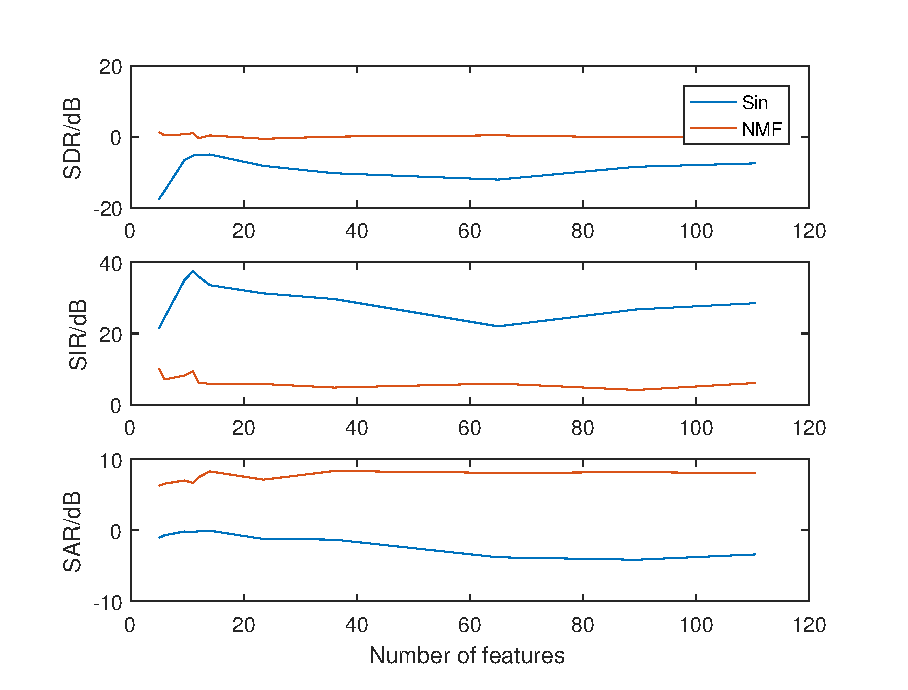
\includegraphics[width=0.7\linewidth]{./FeatureCompPlot}
\caption{Separation performance against the number of features extracted per sound. For the matrix factors, the same number of features were extracted on every input from the set, whereas with sinusoidal trajectories the threshold was constant, giving a range of actual sinusoid quantities so the average was taken.}
\label{fig:FeatureCompPlot}
\end{figure}

\begin{figure}
\centering
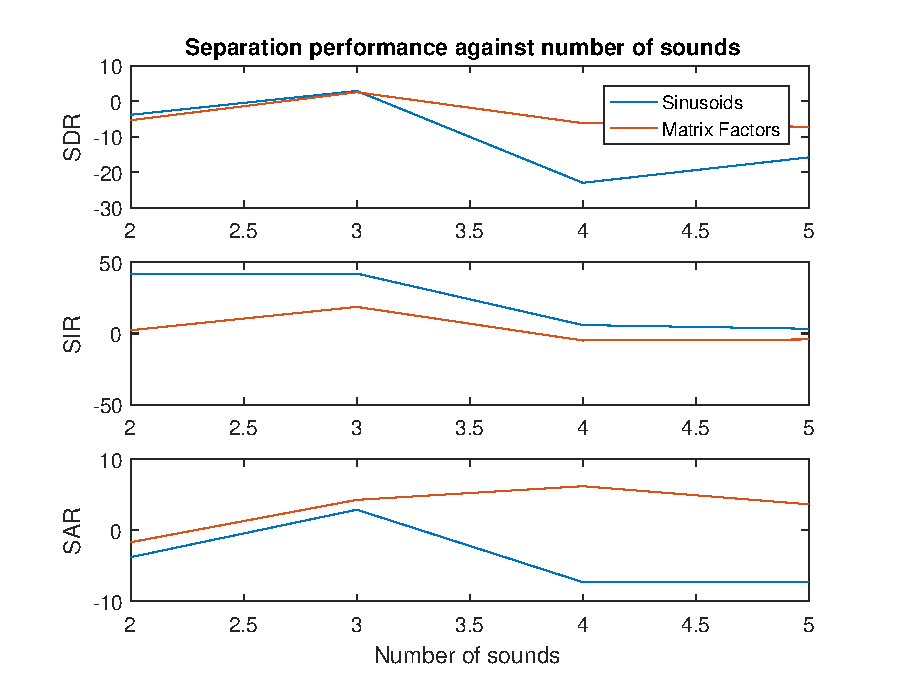
\includegraphics[width=0.7\linewidth]{./FeatureKGraph}
\caption{Separation performance against the number of sounds in the mix. These values were taken over a single example where a complex auditory scene was gradually built up (so the sounds used in each test were also present in all later tests).}
\label{fig:FeatureKGraph}
\end{figure}

%Comment on trends, noting time taken

Both sinusoidal trajectories and spectrogram factors have their theoretical benefits when it comes to separation. In practice, using the matrix factors gives better SDR and SAR values per feature extracted which is as expected since each one is able to potentially capture a significant proportion of the information and it could take many trajectories to represent a given spectrogram to within some error margin. However, the finer control over regions of the spectrogram and the guarantee that each feature originates from a single source (except for the case of colliding harmonics which are much harder to separate in either case) given by the sinusoidal trajectories allow them to generally give SIR values several orders of magnitude larger.

A surprising result is that, with both options, increasing the number of features that were extracted did not always improve the quality of reconstruction or separation. For example, having many ``broken'' trajectories will greatly increase the number of features obtained but most of them will not relate well to one another due to not overlapping for very long in time. This can push the separation towards removing these small artefacts from the mix rather than removing one of the sounds. Also, after obtaining the peaks of the actual harmonics, the next most significant spectral regions are likely to be from spectral leakage around the actual harmonics. These fake sinusoids are unlikely to be clustered with the real sounds since they will not have great harmonic concordance. This latter case is an issue with spectrogram factors as well, since they will eventually start to not actually resemble either of the individual sounds. Given that the time taken for the solution to run increases by a factor of *************** when going from ******** to ********** sinusoidal trajectories, it is often not worth greatly increasing the amount of information used by the system.

When separating sounds from a more complex auditory scene, as in the test used for Figure \ref{fig:FeatureKGraph}, it may be the case that adding another sound to the mix may improve the average quality if the added sound is one that can easily be separated from all others currently present. However, in general the SIR is likely to decrease as the number of sounds increases since there is a much greater likelihood of clashing harmonics. This is reasonable from a human perspective as we will generally struggle in the scenario of the cocktail party problem as the number of simultaneous nearby speakers increases and it would often be a considered a very difficult task to identify the notes played by the third trumpet in a full orchestra.

\subsection{Clustering Method}

%Graphs showing box plots of SDR, SIR, SAR for each clustering method

\begin{figure}
\centering
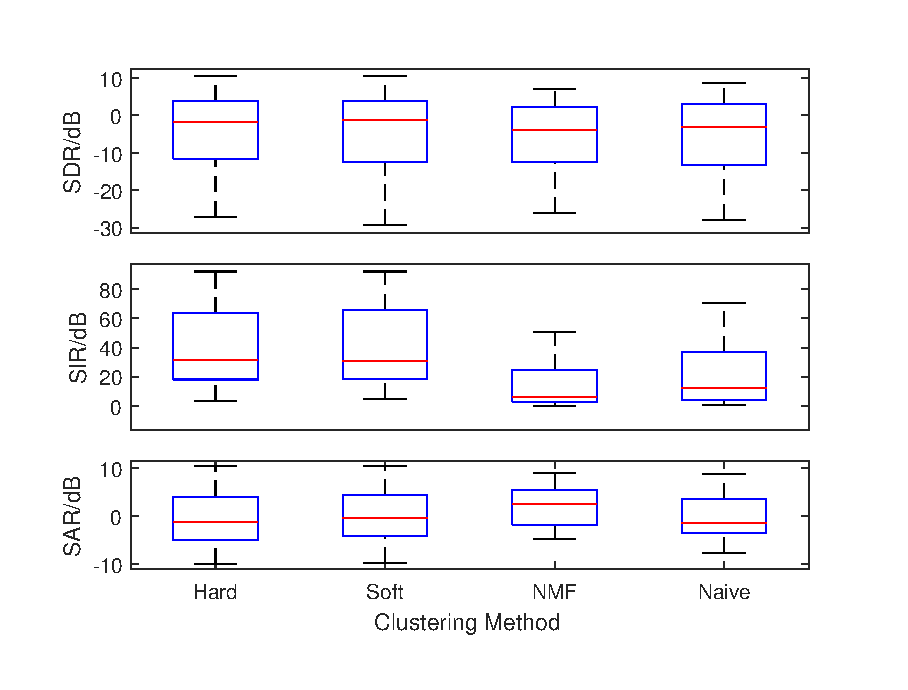
\includegraphics[width=0.7\linewidth]{./ClusteringCompBoxPlotsSin}
\caption{Separation performance against clustering method when using sinusoidal trajectories for the sound elements. These were obtained with only a single test for the soft and NMF clustering options rather than multiple times and taking the ``hardest''.}
\label{fig:ClusteringCompBoxPlotsSin}
\end{figure}

\begin{figure}
\centering
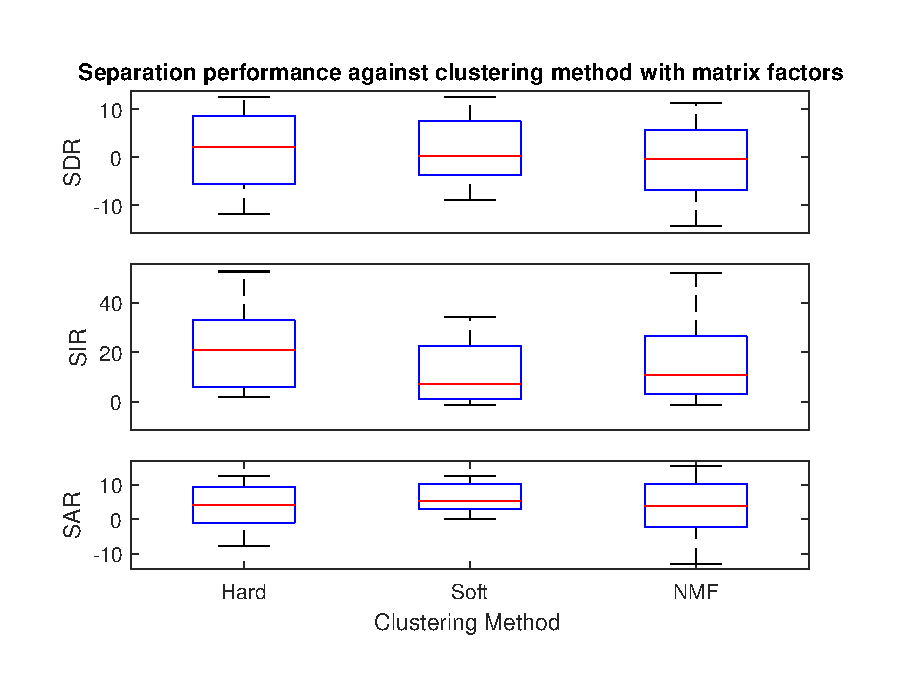
\includegraphics[width=0.7\linewidth]{./ClusteringCompBoxPlotsMat}
\caption{Separation performance against clustering method when using matrix factors for the sound elements.}
\label{fig:ClusteringCompBoxPlotsMat}
\end{figure}

%Comment on trends - best for Sinusoids, best for NMF, intuitions

The expected differences between using the hard and soft $ k $-means clustering methods were that soft clustering would improve the SAR because the reconstructions would be less distorted (misclassified features from the target sound will still be present) at the expense of the SIR (more features from other sounds will be partially present). This was evident in the results when using spectrogram factors. However, I found that there was little difference in the overall quality of the results between using the hard and soft clustering for sinusoidal trajectories. This most likely arose because they were separately optimised for SDR which might have favoured harder assignments for sinusoidal trajectories and softer assignments for spectrogram factors. This may be because of their finer structure ensuring, where possible, that each feature was only from a single sound which can naturally give rise to greater separability and consequently harder assignments.

Theoretically, clustering by NMF should be equivalent to soft $ k $-means but the results show it to act somewhat differently. Due to the lack of ``stiffness'' control when using NMF it would treat the problem the same for both feature options. From the observed results, it would appear as though it is clustering softer than the optimal for sinusoids and harder than the optimal for spectrogram factors.

The na\"{i}ve clustering method was found to offer similar results to the hard and soft $ k $-means but with a lower average SIR. Since it only makes use of the harmonic concordance between sinusoids whereas the other clustering options used a number of different dimensions of comparison, this result comes as no surprise.

From the options presented in this investigation, the results would indicate that using spectrogram factors with soft clustering should be preferred if the purity of the original sounds should be prioritised since it maximises the Signal to Artefact Ratio. On the other hand, the method that looks most promising for accuracy of the separation is by taking the sinusoidal trajectories and separating them by soft clustering.

\subsection{Reversibility}

Describe general effect on SDR, SIR, SAR

\begin{figure}
\centering
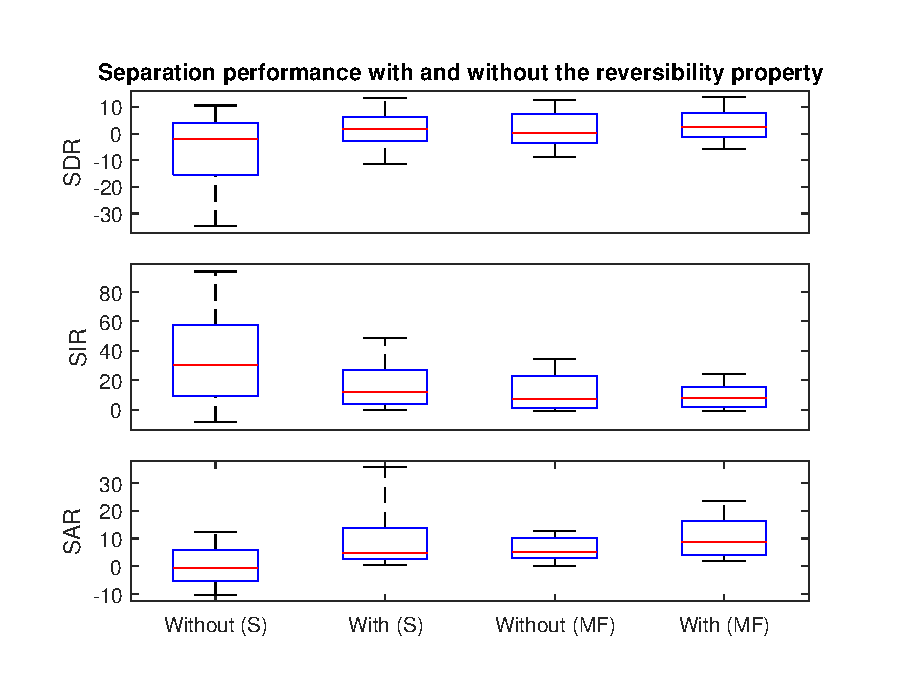
\includegraphics[width=0.7\linewidth]{./ReversibleCompBoxPlots}
\caption{A comparison of the separation performance with and without the reversibility property enforced for each choice of sound element (Sinusoidal trajectories or Matrix Factors).}
\label{fig:ReversibleCompBoxPlots}
\end{figure}

The desired effect of adding the reversibility property is to eliminate artefacts from the combined outputs (and hence some of the artefacts from each individual output). In achieving this, we sacrifice some of the quality of separation by allowing some of the remainder, which may be noise or interference from other sources, to be included in each output. Whilst this is also the intended result of using soft clustering, this can have more dramatic effects, especially in the case where very few features are extracted.

Figure \ref{fig:ReversibleCompBoxPlots} shows the typical effects of enforcing a reversible separation. With both feature options, we obtain a significant increase in SAR as both the artefacts in each output are reduced and the projections onto the target and interference error are increased as the original sounds are better captured. In fact, on this test set the reduction of artefacts was much greater than the increase in interference, giving a higher SDR for some tests that had previously been handled poorly.

\section{Case Analysis}

Describe chosen final solution for further analysis

The remainder of this chapter discusses the performance of the solution against a number of properties of the input. These are primarily targeted at aspects of the solution when using sinusoidal trajectories so we will focus on results acquired with them and soft clustering without forcing reversibility.

\subsection{Performance Against Noise}

%Varying noise level

%Varying threshold without noise

%Graphs showing output SNR, SDR, SAR against input SNR

\begin{figure}
\centering
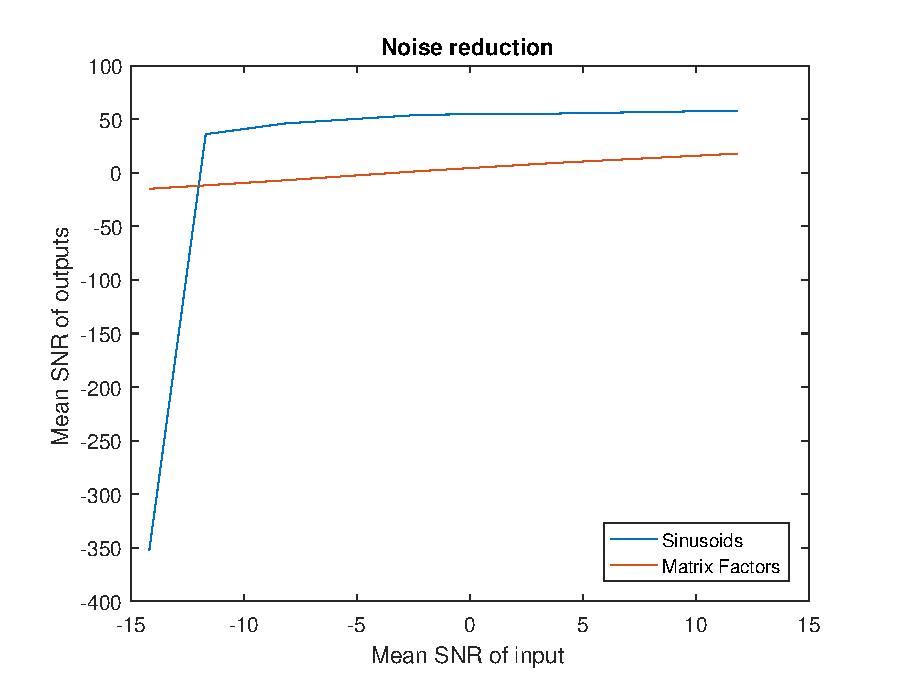
\includegraphics[width=0.7\linewidth]{./NoisePlot}
\caption{Noise reduction at different levels when using both feature options. The standard test set was used but a sample of white noise is added. Since the amplitude of the individual instrument samples vary, the SNR will vary over the inputs and so was averaged for each level of noise.}
\label{fig:NoisePlot}
\end{figure}

%Comment on how much noise is removed/how it affects the artefacts

When modelling the sound using sinusoids, I am explicitly thresholding the STFT at a given level. When the noise sits below that level, none of it will be extracted as features and hence it will not appear in the outputs. However, as we decrease the SNR in the input, some of the noise will start to push over the threshold. This will not only add elements of the noise to the output, but it may cause worse clustering, adding more interference and reducing the level of the target sound. After reaching this point, increasing the noise level further will simply force more of it over the threshold which increases this effect. Since white noise has a flat spectrum, most of it exceeds the threshold at a similar time, causing the catastrophic drop in SNR shown in Figure \ref{fig:NoisePlot}.

On the other hand, the Matrix Factors are designed to extract the most significant patterns in the spectrogram. As white noise was used, we would expect this to have an approximately flat and constant power spectrum which would allow it to be extracted by a single factor. This means that the clustering results are not greatly affected by the noise level. However, since it is unable to eliminate this noise it will always be present in the outputs at approximately the same level as at the input.

\subsection{Performance Against Stereo Separation}

%Graph of SDR, SAR, SIR against stereo difference (two inputs only)

\begin{figure}
\centering
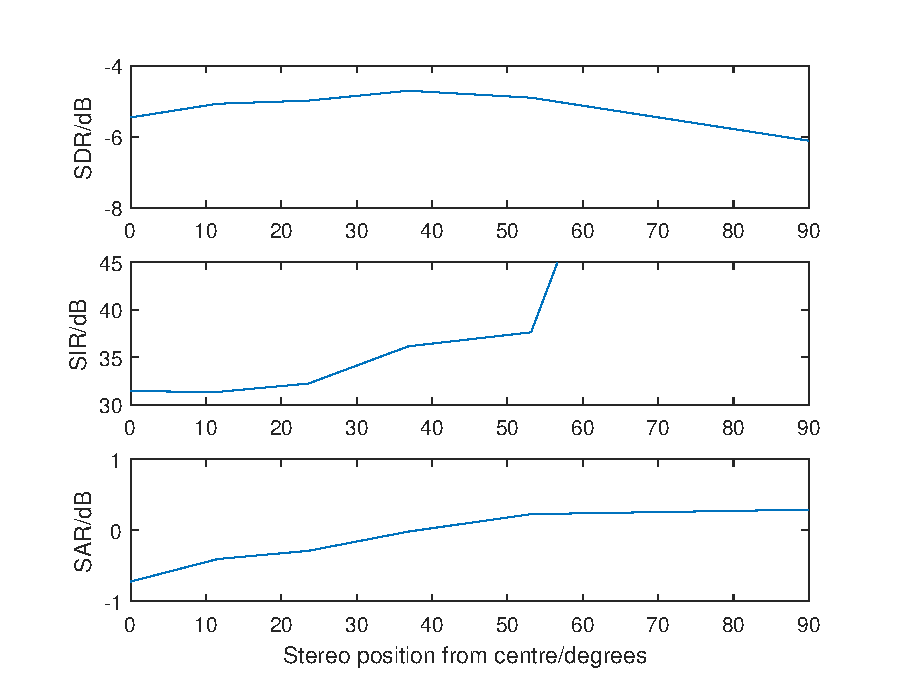
\includegraphics[width=0.7\linewidth]{./StereoPlots}
\caption{Separation performance against the stereo distance between the sounds in the input. These were obtained by using the standard test set but with fixed, as opposed to randomly selected, stereo positions. The stereo position value for a given sound is the proportion of its power routed through the left channel and the distance is the absolute difference between the stereo positions of the two sounds, so $ 0 $ corresponds to the sounds having the same stereo position and $ 1 $ means that they are maximally separated (one is entirely in the left channel and the other is entirely in the right channel).}
\label{fig:StereoPlots}
\end{figure}

A greater stereo distance between two trajectories gives greater confidence that they are from different sources. This is demonstrated by the system as the SIR increases with stereo distance as in Figure \ref{fig:StereoPlots}. One could say that any non-zero stereo distance would indicate that a pair of trajectories are not related but in practice this is not the case. We will generally observe some error in the estimate of the stereo position due to noise and random variations. This means that it would be sensible to allow some tolerance with respect to stereo distance. Furthermore, if the trajectory corresponds to colliding harmonics, the stereo position will not necessarily match that of either source, so we may still wish to consider grouping together trajectories with large stereo distances. This is captured by my system in how the sharp increase in SIR caused by the stereo information dominating occurs at a rather large stereo distance.

\subsection{Performance Against Frequency Offset}

%Graph of SDR, SAR, SIR against frequency offset (square wave plus sine wave)

\begin{figure}
\centering
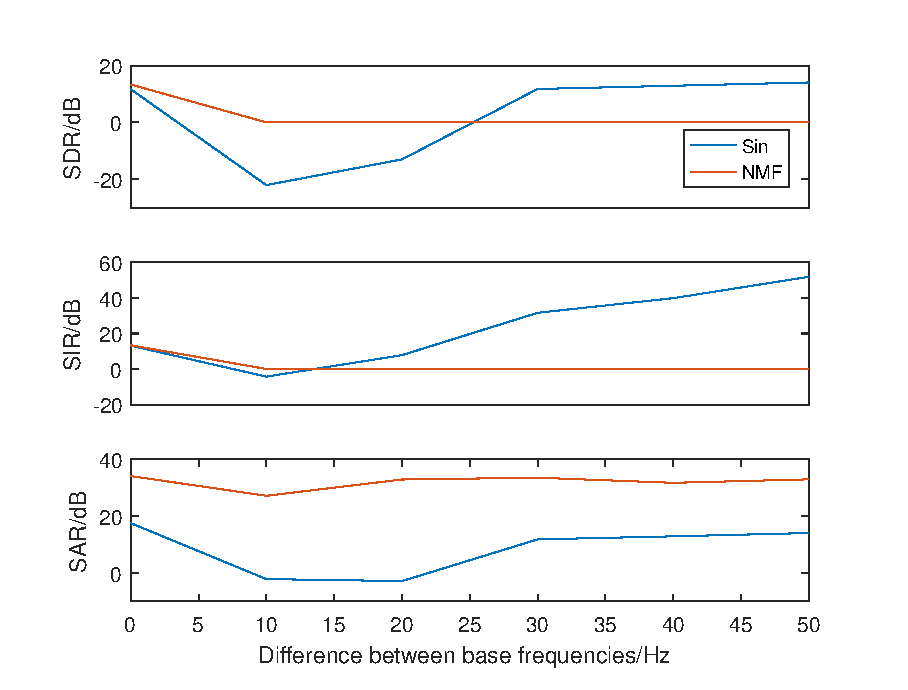
\includegraphics[width=0.7\linewidth]{./FrequencyPlot}
\caption{Separation performance against frequency offset between the sounds. The inputs to this were a $ 465 $Hz square wave and a sine wave at some slightly higher frequency.}
\label{fig:FrequencyPlot}
\end{figure}

The frequency of a sinusoid is important at both the feature extraction and clustering stages of the solution. If the frequencies of two sinusoids are too close together, there is a chance that the STFT peaks caused by one of them might mask the peaks of the other and so it is not extracted at all or, in the extreme case, they collide and so a single trajectory is extracted representing both of them. When two sinusoids are close in frequency, those other sinusoids in harmonic concordance with one are likely to have good concordance with the other, making it harder to notice which one is from which sound. This is demonstrated by the general trend in Figure \ref{fig:FrequencyPlot}. The interesting result from this test was that having the sinusoids collide improved the quality of the outputs, compared to when they are at slightly different frequencies.

%Graph of SDR, SAR, SIR against pitch offset (square wave plus pitch-shifted square wave)

\begin{figure}
\centering
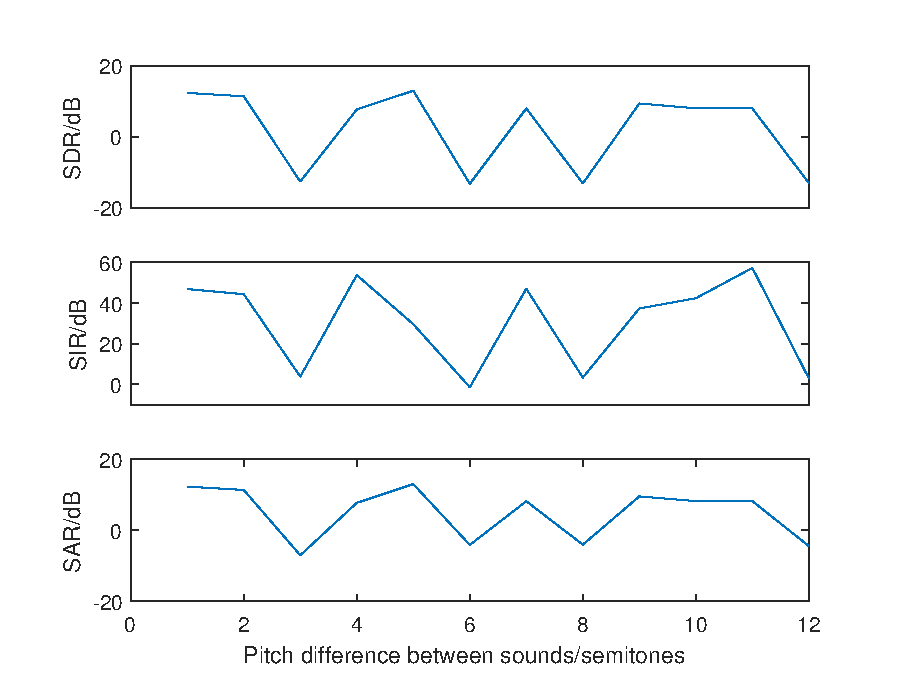
\includegraphics[width=0.7\linewidth]{./PitchPlot}
\caption{Separation performance against pitch offset between the sounds. The input here was a combination of two square waves; one at $ 465 $Hz (approximately corresponding to the MIDI note $ \mathrm{A}^\sharp 4 $) and the other at some number of semitones above.}
\label{fig:PitchPlot}
\end{figure}

The issues with frequency do not only occur when the base frequencies of the sounds are close, but when two sounds happen to harmonise well. Figure \ref{fig:PitchPlot} demonstrates this effect as we observe drastic drops in performance when the inputs have intervals of $ 3 $, $ 6 $, $ 8 $ or $ 12 $ semitones. However, one would expect that intervals of $ 4 $ and $ 7 $ would have particularly poor performance as the ratio of frequencies are approximately $ \frac{5}{4} $ and $ \frac{3}{2} $ whereas those identified are close to $ \frac{6}{5} $, $ \frac{7}{5} $ and $ \frac{8}{5} $ (ignoring the $ \frac{2}{1} $ from the octave). It is unfortunate that the same principle of what makes combinations of musical notes sound appealing also makes them harder to separate.

\subsection{Performance Against Time Offset}

%Graph of SDR, SAR, SIR against time offset (two different instruments, same note, varying time offset)

\begin{figure}
\centering
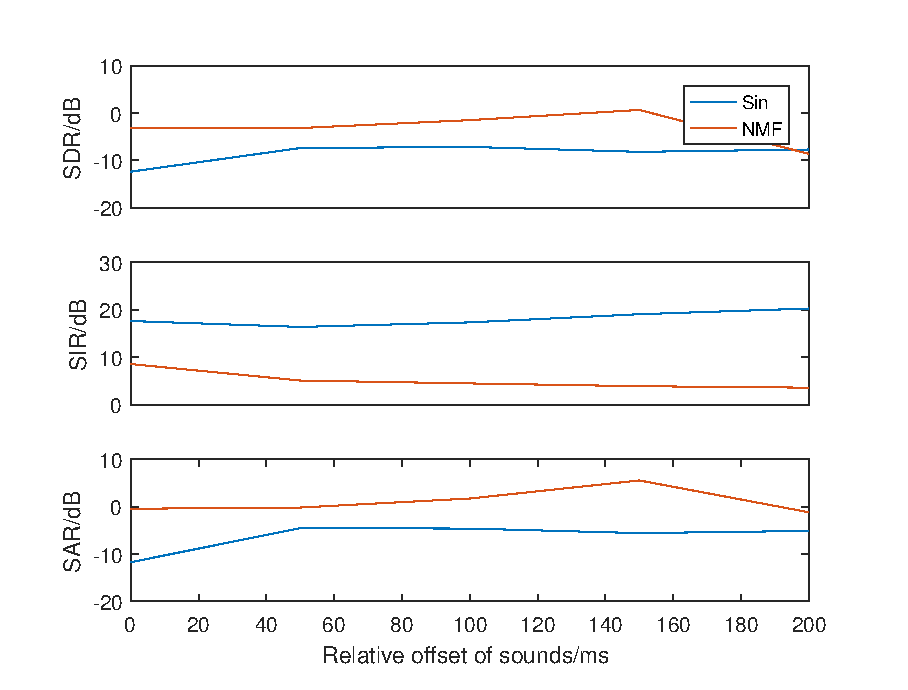
\includegraphics[width=0.7\linewidth]{./OffsetPlot}
\caption{Separation performance against time offset. Two instrument samples were selected from the collection and aligned such that they appeared to be played at the same time. One was then progressively delayed to give the different test inputs.}
\label{fig:OffsetPlot}
\end{figure}

The onsets of the sounds are important in this separation process when using sinusoidal trajectories in the onset distance and in determining the overlapping regions for the frequency, amplitude and stereo envelope distances (in the latter case, the normalisation for the overlap duration should not cause a great difference when varying the onset time slightly). As expected, the solution showed a gradual increase in SIR as the onset distance was increased, but I also observed an improvement in SAR immediately after introducing a small delay between the starts of the sounds.

%\subsection{Synthetic Pathological Cases (if I have time/space)}

%Comment on effect of specifying wrong k

%Frequency crossover test

%Speech (overlay two spoken words from different voices and look at results); comment on how speech is different to instruments

\chapter{Conclusion}

%Paragraph stating tasks completed over project

The main goals of this project were to explore and compare the uses of sinusoidal modelling and Non-negative Matrix Factorisation for extracting features of harmonic sounds in the context of sound separation. Since beginning this investigation I have produced a tool which is capable of using either feature model to separate a simple mixture of harmonic sounds. I have gone on to extend this solution to consider the use of a number of different clustering methods, particularly comparing the application of both hard and soft clustering techniques. I have evaluated the performance of the solution using several metrics and provided some interpretations of these results using insight about the human ability to perform this task and the design of the system.

%Open questions on topic

%Comment on my workflow during project

Concerning the management of this project, I have planned and undergone a substantial research and implementation task involving the design of a small software solution to an academically interesting problem. I maintained a fluid specification as the investigation grew to include multiple degrees of comparison, many of which allowed for improvements in the quality of the solution under several different metrics. Whilst time management was an issue at some points in the project timeline, any setbacks were rectified and the latter half of the work segments were completed to schedule.

%Potential further extensions - UI for assisted clustering, tensor decomposition

Although this dissertation marks the end of the project, there are a few potential improvements on the solution that could still be made. The addition of an interactive user interface for assisted clustering could yield vastly improved separation results as humans are very good at spotting the kinds of patterns that are exhibited in the spectrum of an instrument and for identifying possible issues like colliding harmonics or spectral regions with significant noise or artefacts. I would plan to do this by presenting the spectrogram of the input, highlighting each sinusoidal trajectory according to the cluster to which it is assigned, then allow the user to manually fix the clusters of some trajectories, to which the system can respond by rerunning the clustering procedure and updating the suggestions. Another further extension would be to incorporate stereo information into the extraction of matrix factors by using tensor decomposition (an extension to NMF allowing it to be used on tensors of higher dimensions) or by running NMF on a concatenation of the spectrograms of the left and right channels.

%Use of solutions and state of field

The solution presented here was based on the works of Virtanen and Klapuri \cite{virtanen2000separation} on sound separation by sinusoidal modelling and by NMF \cite{virtanen2003sound} but the state of the art in the field has since moved on. Each of these techniques has been improved on with the introduction of smoothness constraints \cite{virtanen2003algorithm} and High Resolution NMF \cite{badeau2011gaussian}`. More specialised cases have been introduced for human speech which directly tackle the cocktail party problem and the applications of personal assistants and responding to voice-commands. For musically focussed separation, Celemony's Melodyne \cite{melodyne} is a notable leader amongst the commercial solutions, providing suitable quality for most editing and sampling needs. The solution I have presented in this project may not provide the scale of operation that commercial products are capable of, but it demonstrates some of the principles of sound separation that make it feasible to obtain results of a high quality.

\appendix

\chapter{Test Cases}

Include spectrograms of examples of typical test inputs, performance tests and pathological cases

%\chapter{Bibliography}

\bibliography{DissertationBib}

\bibliographystyle{ieeetr}

\chapter{Project Proposal}

Include original proposal

\end{document}